类黄酮是一类带有酚环的天然产物,存在于许多水果与蔬菜中。由于其抗氧化性和抗癌性,类黄酮常用于我们的日常生活。芦丁是一种典型的类黄酮物质,由黄酮醇槲皮苷和二糖芦丁糖构成。

\begin{figure}[h]
	\centering
	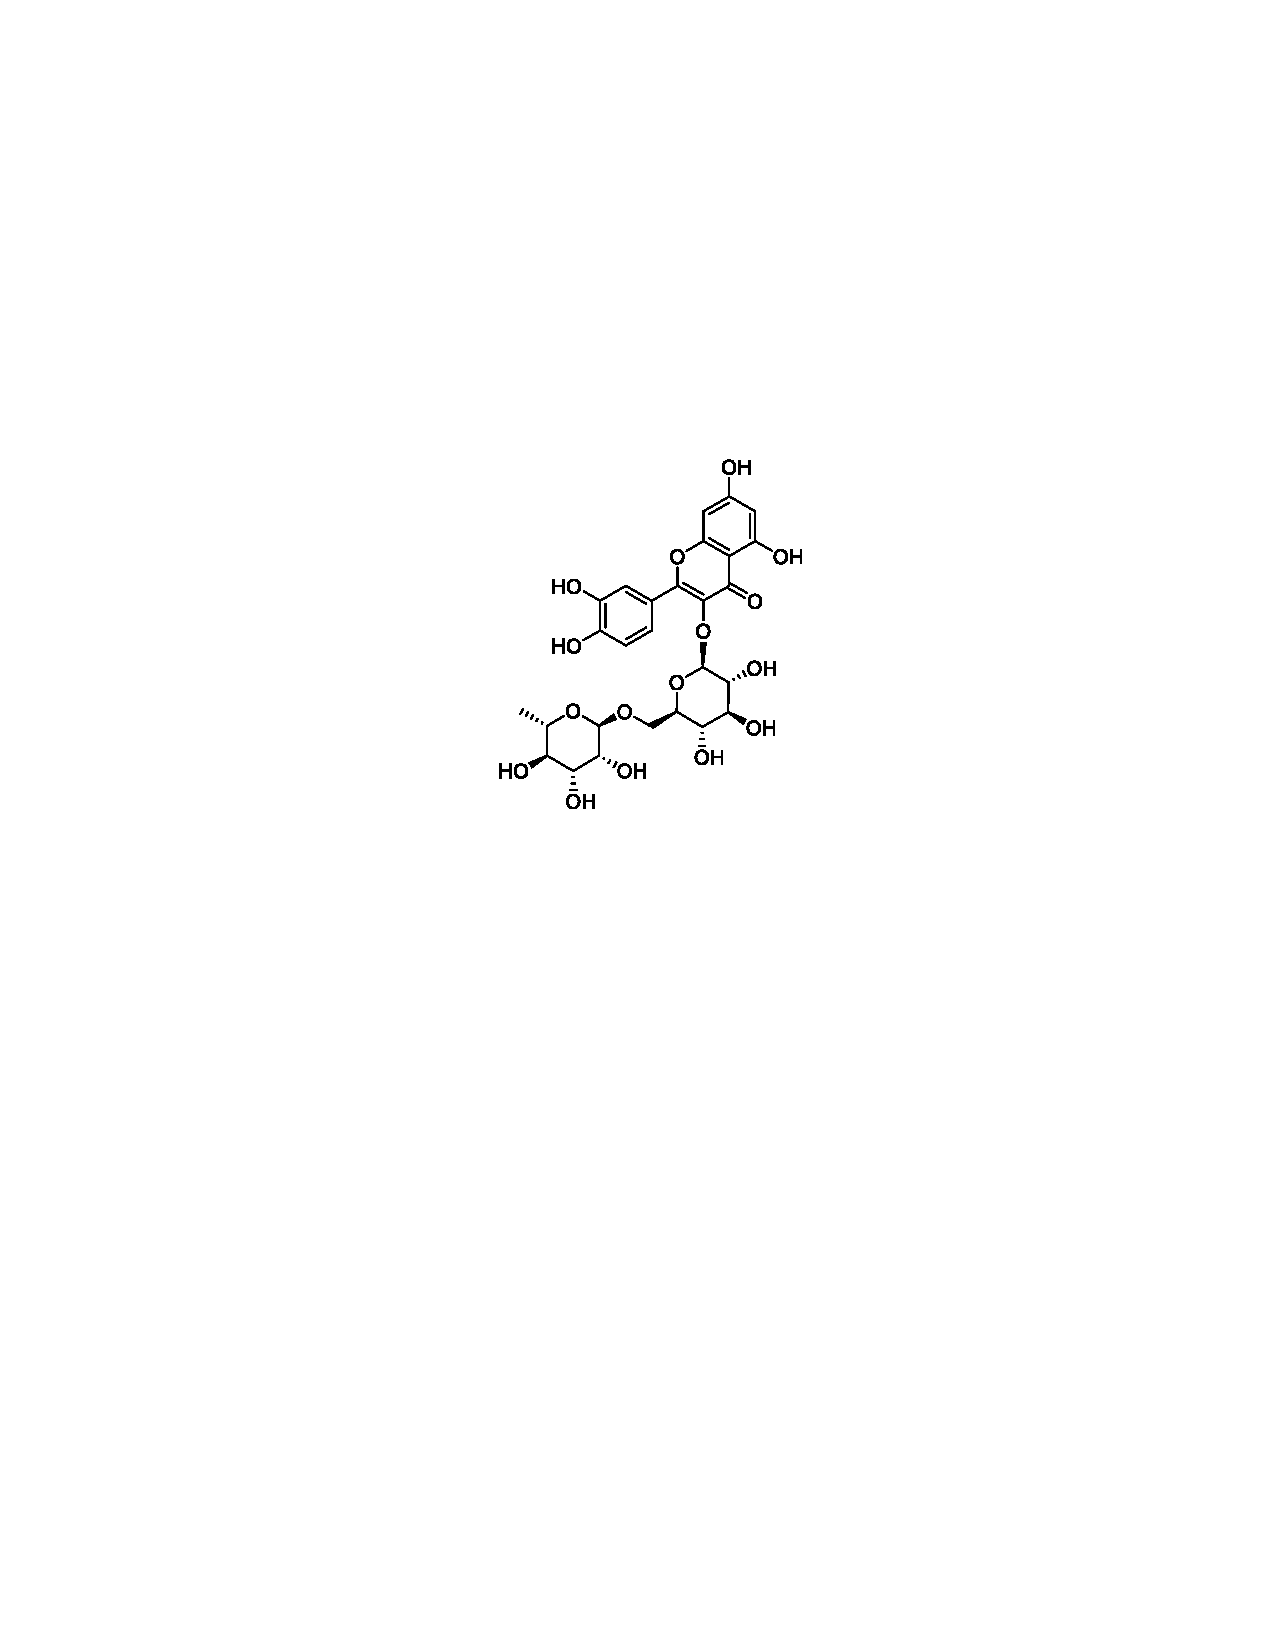
\includegraphics[width=6cm]{./pic/t17-1.pdf}
	\caption*{芦丁的化学结构}
\end{figure}

芦丁对人类健康毒性很低,而且它能向活泼的自由基提供电子以形成更稳定、对健康威胁更小的结构。芦丁还被称作维生素P,其中P是指的它的渗透性。芦丁是一种电化学活性物质许多研究者用不同的电化学技术广泛地研究了它的电化学行为。

循环伏安法是一种有效的电化学测量技术,它将被分析物溶解在电解质溶液中,再向这个电化学电池溶液中插入三根电极:工作电极、对电极和参比电极。由于参比电极具有恒定的电极电势,所以将工作电极与参比电极的电势差进行扫描。工作电极的对电化学反应(译注:reverse electrochemical reactions,如电解水时,产生氢气的电极反应就是产生氧气的电极反应的对电化学反应)发生在对电极上,因此电流在工作电极和对电极之间流动。参比电极则是用来调节工作电极的电势到一个已知的值的。这种技术是基于动态电位的应用。工作电极与参比电极的电势差随时间在两个电势值之间扫描。循环伏安法的应用可以得到电流对扫描电势的图像(伏安图),其中有两个用于评估的重要参数:峰电势和峰电流,它们分别是伏安图的峰对应的$x$轴和$y$轴的值。

用玻碳电极、饱和甘汞电极(SCE)和Pt丝分别作为工作电极、参比电极和对电极,测试了芦丁25 °C下的循环伏安(CV)特性。在这项研究中,以100 mV s\textsuperscript{−1}的扫描速率在0.00和0.80 V之间扫描电势,得到了不同pH的1.0×10\textsuperscript{−4} mol dm\textsuperscript{−3}芦丁溶液的CV数据。不同pH下的CV图中的阳极峰电势($E_{p_c}$)、阴极峰电势($E_{p_c}$ )、阳极峰电流($I_{p_a}$)和阴极峰电流($I_{p_c}$)展示在下表中。

\textbf{表} 不同pH的1.0 × 10\textsuperscript{−4} mol
dm\textsuperscript{−3}芦丁溶液的CV数据

此处无CV数据表

\noindent\textbf{17.1.}
在一个三电极体系中,被分析物在电化学电池中的电化学氧化反应和还原反应发生在\_\_\_\_\_上,因为它的电势是根据\_\_\_\_\_调节的。

下列哪组词适合填在上面句子的空里?

a) 工作电极/参比电极

b) 对电极/工作电极

c) 参比电极/工作电极

d) 工作电极/对电极

\noindent\textbf{17.2.} 随着pH的升高,阳极峰电势和阴极峰电势的数值都降低了,因为\_\_\_\_\_参与了芦丁的电化学反应。

下列哪个词适合填在上面句子的空里?

a) Na\textsuperscript{+}

b) K\textsuperscript{+}

c) H\textsuperscript{+}

d) I\textsuperscript{−}

\noindent\textbf{17.3.} 芦丁的电化学氧化反应是\_\_\_\_\_,因为$I_{p_a}/T_{p_c}$约等于1,而且$\Delta E_p$约等于$0.0592/n$ V。

下列哪个词适合填在上面句子的空里?

a) 不可逆的

b) 可逆的

c) 准可逆的

d) 催化的

\noindent\textbf{17.4.} 得到每组CV数据需要多长时间?

\noindent\textbf{17.5.} 计算2个H\textsuperscript{+}参与的芦丁的电化学反应转移的电子数。

\noindent\textbf{17.6.} 给芦丁的电化学氧化还原建议一个机理。

\noindent\textbf{17.7.} SCE的反应是$\ce{Hg2Cl2(s) + 2e^- -> 2Hg(l) + 2Cl^-}$,而且含有饱和KCl溶液:将342 g KCl溶于1.0 L水中。请问相较在1.0 M KCl的情况下,SCE的电势怎样变化(降低或升高)?

为了测定一种维生素P片中芦丁的含量,采取了以下措施:

\textbf{i)} 将一片500 mg的维生素P片溶于去离子水中,调节pH至2.0,在500
mL容量瓶中定容。转移10
mL该溶液至一个三电极电池中,得到CV图:阳极峰电流($I_{p_a}$)为2.26
μA。

\textbf{ii)}
配置一份不含芦丁的pH为2.0的溶液,插入所有的电极,记录下三次实验的CV图,每次测量前都用去离子水清洁电极。$I_{p_a}$值分别为0.16,0.11和0.18 μA。

\textbf{iii)} 配置1.0,5.0,10.0,20.0,30.0和50.0 mM芦丁标准溶液,从这些溶液的CV图得到它们的$I_{p_a}$值,展示在下表中。

\textbf{表} 不同芦丁标准溶液的\emph{I}p\textsubscript{a}值

此处无$I_{p_a}$值表

注意,所有的CV图都是使用相同的工作电极获得的。

\noindent\textbf{17.8.} 画出芦丁测定方法的校准曲线。

\noindent\textbf{17.9.} 写出校准曲线的解析式。

\noindent\textbf{17.10.} 计算维生素P片的芦丁含量,结果用wt\%表示。

\noindent\textbf{17.11.} 用3.0的信噪比(S/N)计算这个方法的灵敏度和检测限(LOD)。

\noindent\textbf{注:}检测限:$\mathrm{LOD}=\frac{k\times s_{\mathrm{blank}}}{m}$
